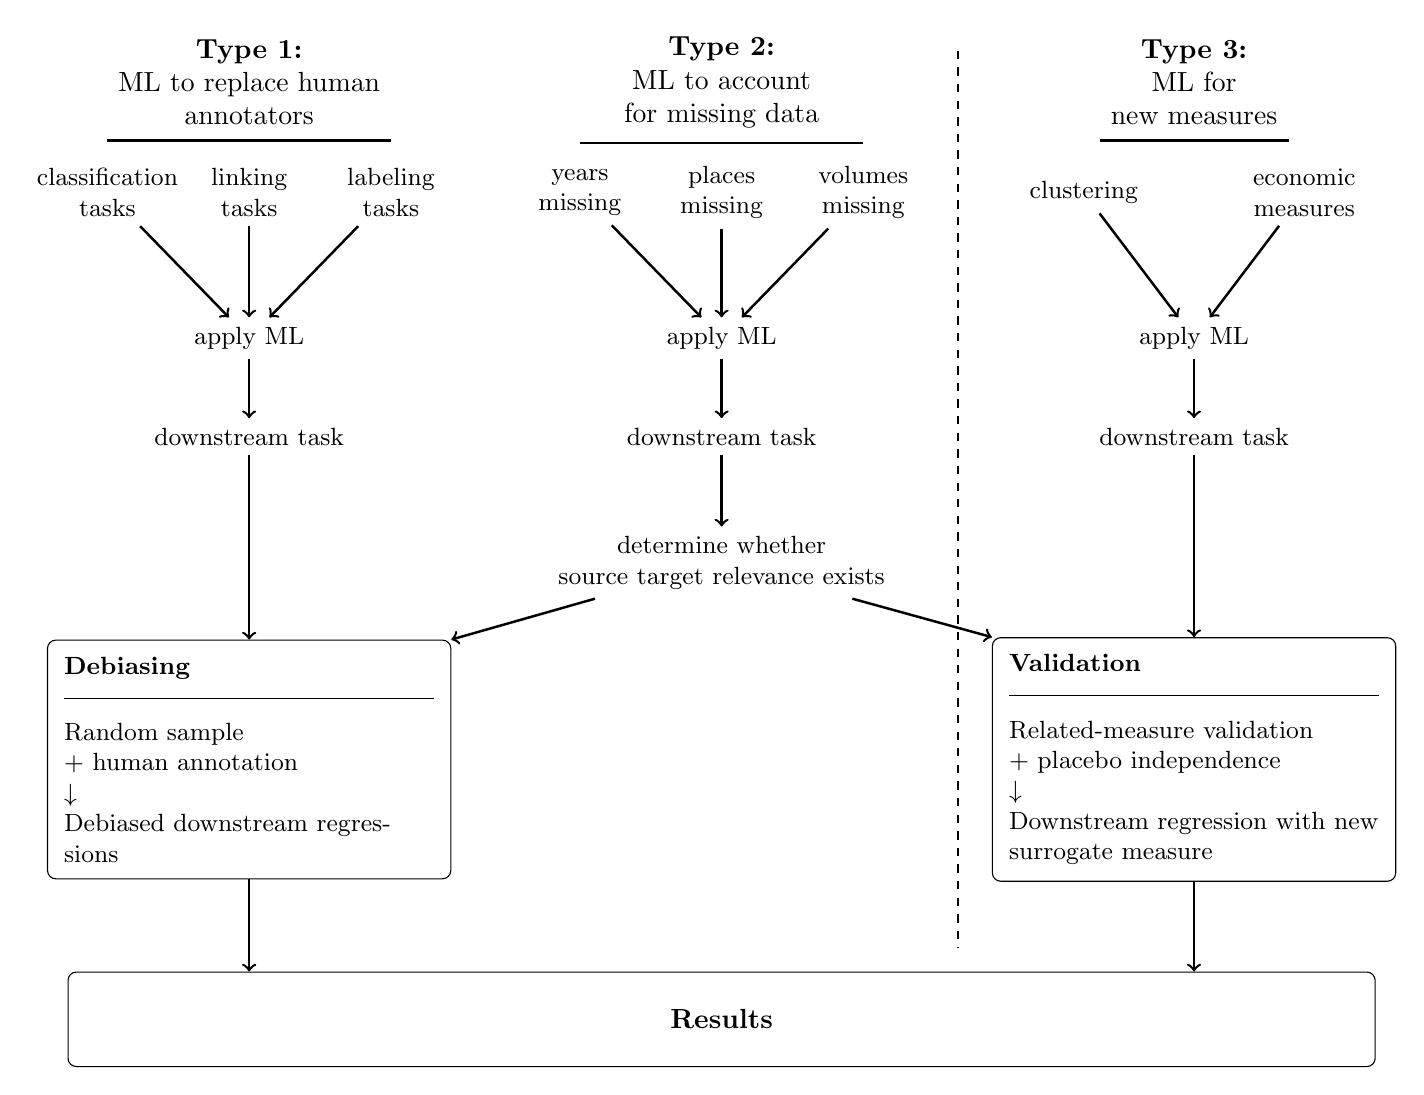
\begin{tikzpicture}[
  font=\normalsize,
  arr/.style={->, line width=0.9pt},
  hdr/.style={align=center},
  small/.style={font=\small, align=center},
  mid/.style={font=\small, align=center},
  box/.style={
    draw,
    rounded corners=3pt,
    align=left,
    inner sep=6pt,
    text width=4.7cm,
    font=\small
  },
  resultsbox/.style={
    draw,
    rounded corners=3pt,
    align=center,
    inner sep=10pt,
    minimum height=1.2cm,
    minimum width=16.6cm
  }
]

% -------------------------------------------------
% Column x-positions
% -------------------------------------------------
\def\xL{-6}
\def\xM{0}
\def\xR{6}

% -------------------------------------------------
% HEADINGS
% -------------------------------------------------
\node[hdr] (h1) at (\xL,0) {\textbf{Type 1:}\\ ML to replace human\\annotators};
\node[hdr] (h2) at (\xM,0) {\textbf{Type 2:}\\ ML to account\\for missing data};
\node[hdr] (h3) at (\xR,0) {\textbf{Type 3:}\\ML for \\new measures};

\draw[line width=0.9pt] (h1.south) ++(-1.8cm,-2pt) -- ++(3.6cm,0);
\draw[line width=0.9pt] (h2.south) ++(-1.8cm,-2pt) -- ++(3.6cm,0);
\draw[line width=0.9pt] (h3.south) ++(-1.2cm,-2pt) -- ++(2.4cm,0);

% -------------------------------------------------
% Dashed separator between (left+middle) and right
% -------------------------------------------------
\draw[dashed, line width=0.9pt] (3,0.4) -- (3,-11.0);

% -------------------------------------------------
% INPUT LABELS
% -------------------------------------------------
\node[small] (c1a) at (\xL-1.8,-1.4) {classification\\tasks};
\node[small] (c1b) at (\xL,-1.4) {linking\\tasks};
\node[small] (c1c) at (\xL+1.8,-1.4) {labeling\\tasks};

\node[small] (c2a) at (\xM-1.8,-1.4) {years\\missing};
\node[small] (c2b) at (\xM,-1.4) {places\\missing};
\node[small] (c2c) at (\xM+1.8,-1.4) {volumes\\missing};

\node[small] (c3a) at (\xR-1.4,-1.4) {clustering};
\node[small] (c3b) at (\xR+1.4,-1.4) {economic\\measures};

% -------------------------------------------------
% ML layer + downstream task layer
% -------------------------------------------------
\node[mid] (ml1) at (\xL,-3.25) {apply ML};
\node[mid] (ds1) at (\xL,-4.5) {downstream task};

\node[mid] (ml2) at (\xM,-3.25) {apply ML};
\node[mid] (ds2) at (\xM,-4.5) {downstream task};

\node[mid] (ml3) at (\xR,-3.25) {apply ML};
\node[mid] (ds3) at (\xR,-4.5) {downstream task};

% -------------------------------------------------
% Type 2: intermediate relevance check
% -------------------------------------------------
\node[mid] (rel2) at (\xM,-6.1) {determine whether\\source target relevance exists};

% -------------------------------------------------
% DE-BIASING BOX (left)
% -------------------------------------------------
\node[box] (b1) at (\xL,-8.6) {
\textbf{Debiasing}\\[-2pt]
\rule{\linewidth}{0.4pt}\\[4pt]
Random sample\\
+ human annotation\\
$\downarrow$\\
Debiased downstream regressions
};

% -------------------------------------------------
% VALIDATION BOX (right)
% -------------------------------------------------
\node[box] (b3) at (\xR,-8.6) {
\textbf{Validation}\\[-2pt]
\rule{\linewidth}{0.4pt}\\[4pt]
Related-measure validation\\
+ placebo independence\\
$\downarrow$\\
Downstream regression with new surrogate measure
};
% -------------------------------------------------
% RESULTS BOX
% -------------------------------------------------
\node[resultsbox] (RES) at (0,-11.9) {\textbf{Results}};

% -------------------------------------------------
% ARROWS
% -------------------------------------------------
% Inputs -> apply ML method
\draw[arr] (c1a) -- (ml1);
\draw[arr] (c1b) -- (ml1);
\draw[arr] (c1c) -- (ml1);

\draw[arr] (c2a) -- (ml2);
\draw[arr] (c2b) -- (ml2);
\draw[arr] (c2c) -- (ml2);

\draw[arr] (c3a) -- (ml3);
\draw[arr] (c3b) -- (ml3);

% apply ML method -> downstream task
\draw[arr] (ml1) -- (ds1);
\draw[arr] (ml2) -- (ds2);
\draw[arr] (ml3) -- (ds3);

% Type 1 and Type 3: downstream task -> boxes
\draw[arr] (ds1) -- (b1.north);
\draw[arr] (ds3) -- (b3.north);

% Type 2: downstream task -> relevance check -> de-biasing and validation
\draw[arr] (ds2) -- (rel2);
\draw[arr] (rel2) -- (b1.north east);
\draw[arr] (rel2) -- (b3.north west);

% -------------------------------------------------
% Targets on the top edge of the Results box
% -------------------------------------------------
\coordinate (t1) at (RES.north -| b1);
\coordinate (t3) at (RES.north -| b3);

% Boxes -> Results
\draw[arr] (b1.south) -- (t1);
\draw[arr] (b3.south) -- (t3);

\end{tikzpicture}